% Section content template for individual Educative lessons
% This file contains the actual content for a specific section
% Generated from Educative API section content

% Section: High-Level Design of a Distributed Cache
% Section ID: 5103962818084864
% Section Slug: high-level-design-of-a-distributed-cache
% Generated: 2025-12-07T20:14:48.059101

In this lesson, we'll learn to design a distributed cache. We 'll also discuss the trade-offs and design choices that can occur while we progress in our journey towards developing a solution.

\subsection{Requirements}\label{hObkOv7XLstdQpVCxeWQg}
\\
Let us start by understanding the requirements of our solution.

\subsubsection{Functional}\label{-aMIq4x-0mgXwJkAraNDQ}
\\
The following are the functional requirements:

\begin{itemize}
\item
\protect\phantomsection\label{zCBiurHiEbGbjtGA0uWBw}
\textbf{Insert data:} The user of a distributed cache system must be able to insert an entry to the cache.
\item
\protect\phantomsection\label{B8vA203Nz-ldzQ1azt_Gv}
\textbf{Retrieve data:} The user should be able to retrieve data corresponding to a specific key.
\end{itemize}

\begin{figure}[htbp]
 \centering
 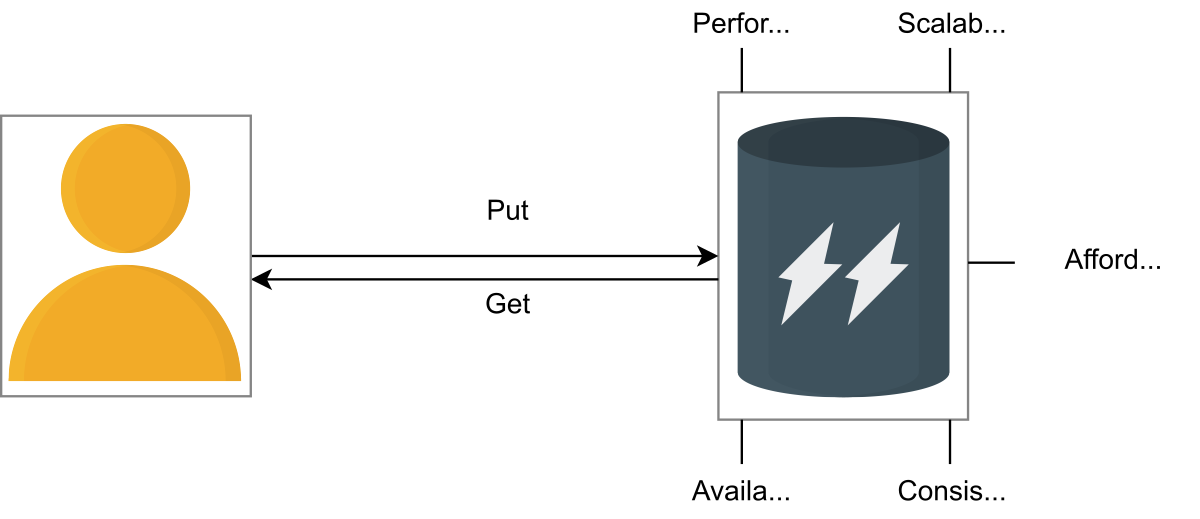
\includegraphics[width=0.5\textwidth]{Images/chapter_16/section_5103962818084864/5256732863627264.png}
 \caption{Functional and non-functional requirements of a distributed cache}
\end{figure}

\subsubsection{Non-functional requirements}\label{DFwvX42KfV2rkbCDIm30G}
\\
We'll consider the following non-functional requirements:

\begin{itemize}
\item
\protect\phantomsection\label{0g8UkxyDuXHnGOLwgsM_D}
\textbf{High performance}: The primary reason for the cache is to enable fast retrieval of data. Therefore, both the \texttt{insert} and \texttt{retrieve} operations must be fast.
\item
\protect\phantomsection\label{1kXHUfgyLFhLz2bktb9dg}
\textbf{Scalability:} The cache system should scale horizontally with no bottlenecks on an increasing number of requests.
\item
\protect\phantomsection\label{IELRkO7oeLqKU9stf8gnU}
\textbf{High availability}: The unavailability of the cache will put an extra burden on the database servers, which can also go down at peak load intervals. We also require our system to survive occasional failures of components and network, as well as power outages.
\item
\protect\phantomsection\label{0SqpxWahCzer30DFiWwTR}
\textbf{Consistency:} Data stored on the cache servers should be consistent. For example, different cache clients retrieving the same data from different cache servers (primary or secondary) should be up to date.
\item
\protect\phantomsection\label{nvI_V1IRk8pN4zyY6AOu_}
\textbf{Affordability:} Ideally, the caching system should be designed from commodity hardware instead of an expensive supporting component within the design of a system.
\end{itemize}

\subsection{API design}\label{9xj--dRijmEBp8cJ54_6f}
\\
The API design for this problem is sufficiently easy since there are only two basic operations.

\subsubsection{Insertion}\label{qrluScoAPjJDMhBBBmm4a}
\\
The API call to perform insertion should look like this:

\begin{lstlisting}[language=JavaScript]
insert(key, value)
\end{lstlisting}

\begin{table}[htbp]
\centering
\small
\adjustbox{max width=\textwidth}{
\begin{tabular}{|p{0.340\textwidth}|p{0.610\textwidth}|}
\hline
\textbf{Parameter} & \textbf{Description} \\
\hline
\hline
\texttt{key} & This is a unique identifier. \\
\hline
\texttt{value} & This is the data stored against a unique \texttt{key}. \\
\hline
\end{tabular}
}
\end{table}

This function returns an acknowledgment or an error depicting the problem at the server end.

\subsubsection{Retrieval}\label{BZKUGbhuKmK_hr2Qsab20}
\\
The API call to retrieve data from the cache should look like this:

\begin{lstlisting}[language=JavaScript]
retrieve(key)
\end{lstlisting}

\begin{table}[htbp]
\centering
\small
\adjustbox{max width=\textwidth}{
\begin{tabular}{|p{0.340\textwidth}|p{0.610\textwidth}|}
\hline
\textbf{Parameter} & \textbf{Description} \\
\hline
\hline
\texttt{key} & This returns the data stored against the \texttt{key.} \\
\hline
\end{tabular}
}
\end{table}

This call returns an object to the caller.

\begin{quote}
\textbf{Quiz:}
\textbf{Question 1:} The API design of the distributed cache looks exactly like the key-value store. What are the possible differences between a key-value store and a distributed cache?
\textbf{Answer:} Some of the key differences are the following: - Key-value stores need to durably store data (persistence). A cache is used in addition to persistent storage to increase reading performance. - A cache serves data from the RAM. A key-value store writes data to non-volatile storage. - Key-value stores are robust and should survive failures.

However, caches can crash and be populated from scratch after recovery.
\end{quote}

\subsection{Design considerations}\label{0H4nfElXUHpzu20mRlcXD}
\\
Before designing the distributed cache system, it's important to consider some design choices. Each of these choices will be purely based on our application requirements. However, we can highlight some key differences here:

\subsubsection{Storage hardware}\label{aqgrB7cgEFZOlEELkm-Km}
\\
If our data is large, we may require sharding and therefore use shard servers for cache partitions. Should these shard servers be specialized or commodity hardware? Specialized hardware will have good performance and storage capacity, but it will cost more. We can build a large cache from commodity servers(Facebook built 28 TeraBytes of cache using commodity machines in 2013.). In general, the number of shard servers will depend on the cache's size and access frequency.
\\
Furthermore, we can consider storing our data on the secondary storage of these servers for persistence while we still serve data from RAM. Secondary storage may be used in cases where a reboot happens, and cache rebuilding takes a long time. Persistence , however, may not be a requirement in a cache system if there's a dedicated persistence layer, such as a database.

\subsubsection{Data structures}\label{snn0_SpaUMXYgs1FM8h2z}
\\
A vital part of the design has to be the speed of accessing data. Hash tables are data structures that take a constant time on average to store and retrieve data. Furthermore , we need another data structure to enforce an eviction algorithm on the cached data. In particular, linked lists are a good option (as discussed in the previous lesson).
\\
Also, we need to understand what kind of data structures a cache can store. Even though we discussed in the API design section that we'll use strings for simplicity, it's possible to store different data structures or formats, like hash maps, arrays, sets, and so on, within the cache. In the next lesson, we'll see a practical example of such a cache.

\subsubsection{Cache client}\label{eikN-V5MVLo9S1FpxMez8}
\\
It's the client process or library that places the \texttt{insert} and \texttt{retrieve} calls. The location of the client process is a design issue. For example, it's possible to place the client process within a serving host if the cache is for internal use only. Otherwise , in the case where the caching system is provided as a service for external use, a dedicated cache client can send users' requests to the cache servers.

\subsubsection{Writing policy}\label{gZpJMYaWE01Nm2mAGOZol}
\\
The writing strategy over the cache and database has consistency implications. In general, there's no optimal choice, but depending on our application, the preference of writing policy is significantly important.

\subsubsection{Eviction policy}\label{rCnXfAN6ypmaJr57Z_tEK}
\\
By design, the cache provides low-latency reads and writes. To achieve this, data is often served from RAM memory. Usually , we can't put all the data in the cache due to the limited size of the cache as compared to the full dataset. So
, we need to carefully decide what stays in the cache and how to make room for new entries.
\\
With the addition of new data, some of the existing data may have to be evicted from the cache. However, choosing a victim entry depends on the eviction policy. Numerous eviction policies exist, but the choice again depends on the application using it. For instance, least recently used (LRU) can be a good choice for social media services where recently uploaded content will likely get the most views.
\\
Apart from the details in the sections above, optimizing the time-to-live (TTL) value can play an essential role in reducing the number of cache misses.
\\
How does sharding help mitigate single points of failure (SPOF) in a distributed cache system?
\\
Use the AI assessment widget below to submit your solution and get an interactive response.

\textbf{Question:}

How can sharding help eliminate SPOFs?

\textbf{Reference Answer:}

Sharding involves dividing the cache data into smaller, manageable chunks (shards) and distributing them across multiple cache servers. This approach mitigates single points of failure (SPOFs) by ensuring that each shard is stored on a different server. If one server fails, only the data on the affected shard is lost, while the rest of the system remains intact.

\subsection{High-level design}\label{LAlGMPZW6372bCFLdXYra}
\\
The following figure depicts our high-level design:

\begin{figure}[htbp]
 \centering
 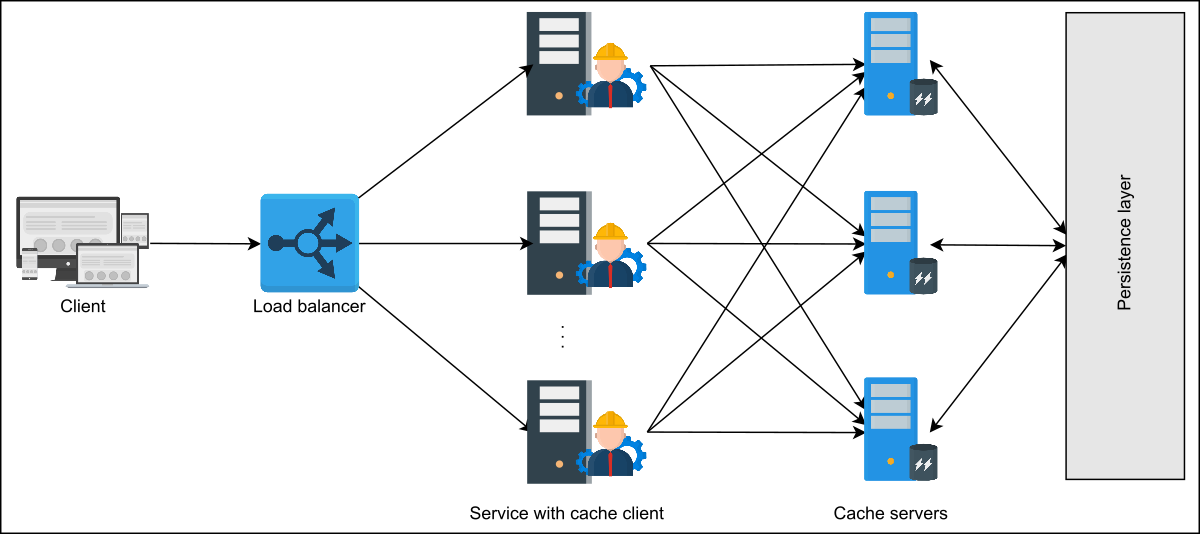
\includegraphics[width=0.5\textwidth]{Images/chapter_16/section_5103962818084864/5777399426056192.png}
 \caption{High-level design of distributed cache}
\end{figure}

The main components in this high-level design are the following:

\begin{itemize}
\item
\protect\phantomsection\label{FaXbl531nrtCu7YbWIdqS}
\textbf{Cache client}: This library resides in the service application servers. It holds all the information regarding cache servers. The cache client will choose one of the cache servers using a hash and search algorithm for each incoming \texttt{insert} and \texttt{retrieve} request. All the cache clients should have a consistent view of all the cache servers. Also, the resolution technique to move data to and from the cache servers should be the same. Otherwise, different clients will request different servers for the same data.
\item
\protect\phantomsection\label{ZAoBgN3bYFVXR04O10KBK}
\textbf{Cache servers}: These servers maintain the cache of the data. Each cache server is accessible by all the cache clients. Each server is connected to the database to store or retrieve data. Cache clients use TCP or UDP protocol to perform data transfer to or from the cache servers. However, if any cache server is down, requests to those servers are resolved as a missed cache by the cache clients.
\end{itemize}

% End of section content